\section{mo\-Linear\-Cooling\-Schedule Class Reference}
\label{classmo_linear_cooling_schedule}\index{moLinearCoolingSchedule@{moLinearCoolingSchedule}}
One of the possible {\bf mo\-Cooling\-Schedule}{\rm (p.\,\pageref{classmo_cooling_schedule})}.  


{\tt \#include $<$mo\-Linear\-Cooling\-Schedule.h$>$}

Inheritance diagram for mo\-Linear\-Cooling\-Schedule::\begin{figure}[H]
\begin{center}
\leavevmode
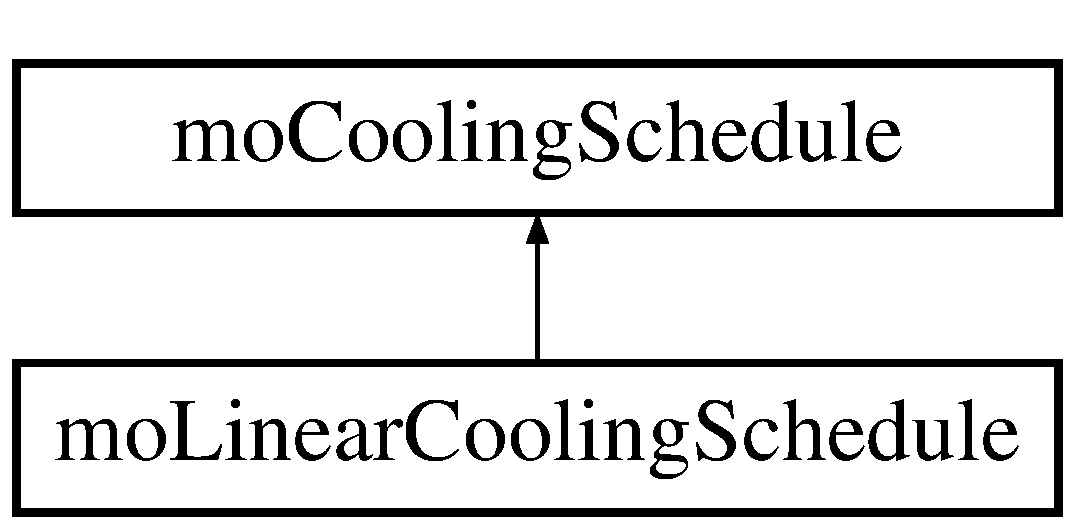
\includegraphics[height=4cm]{classmo_linear_cooling_schedule}
\end{center}
\end{figure}
\subsection*{Public Member Functions}
\begin{CompactItemize}
\item 
{\bf mo\-Linear\-Cooling\-Schedule} (double \_\-threshold, double \_\-quantity)
\begin{CompactList}\small\item\em Simple constructor. \item\end{CompactList}\item 
bool {\bf operator()} (double \&\_\-current\_\-temperature)
\begin{CompactList}\small\item\em Function which proceeds to the cooling. \item\end{CompactList}\end{CompactItemize}
\subsection*{Private Attributes}
\begin{CompactItemize}
\item 
double {\bf threshold}\label{classmo_linear_cooling_schedule_r0}

\begin{CompactList}\small\item\em The temperature threhold. \item\end{CompactList}\item 
double {\bf quantity}\label{classmo_linear_cooling_schedule_r1}

\begin{CompactList}\small\item\em The quantity that allows the temperature to decrease. \item\end{CompactList}\end{CompactItemize}


\subsection{Detailed Description}
One of the possible {\bf mo\-Cooling\-Schedule}{\rm (p.\,\pageref{classmo_cooling_schedule})}. 

An another very simple cooling schedule, the temperature decrease according to a quantity while the temperature is greater than a threshold. 



Definition at line 46 of file mo\-Linear\-Cooling\-Schedule.h.

\subsection{Constructor \& Destructor Documentation}
\index{moLinearCoolingSchedule@{mo\-Linear\-Cooling\-Schedule}!moLinearCoolingSchedule@{moLinearCoolingSchedule}}
\index{moLinearCoolingSchedule@{moLinearCoolingSchedule}!moLinearCoolingSchedule@{mo\-Linear\-Cooling\-Schedule}}
\subsubsection{\setlength{\rightskip}{0pt plus 5cm}mo\-Linear\-Cooling\-Schedule::mo\-Linear\-Cooling\-Schedule (double {\em \_\-threshold}, double {\em \_\-quantity})\hspace{0.3cm}{\tt  [inline]}}\label{classmo_linear_cooling_schedule_a0}


Simple constructor. 

\begin{Desc}
\item[Parameters:]
\begin{description}
\item[{\em \_\-threshold}]the threshold. \item[{\em \_\-quantity}]the quantity used to descrease the temperature. \end{description}
\end{Desc}


Definition at line 55 of file mo\-Linear\-Cooling\-Schedule.h.

References quantity, and threshold.

\subsection{Member Function Documentation}
\index{moLinearCoolingSchedule@{mo\-Linear\-Cooling\-Schedule}!operator()@{operator()}}
\index{operator()@{operator()}!moLinearCoolingSchedule@{mo\-Linear\-Cooling\-Schedule}}
\subsubsection{\setlength{\rightskip}{0pt plus 5cm}bool mo\-Linear\-Cooling\-Schedule::operator() (double \& {\em \_\-current\_\-temperature})\hspace{0.3cm}{\tt  [inline, virtual]}}\label{classmo_linear_cooling_schedule_a1}


Function which proceeds to the cooling. 

It decreases the temperature and indicates if it is greater than the threshold.

\begin{Desc}
\item[Parameters:]
\begin{description}
\item[{\em \_\-current\_\-temperature}]The current temperature. \end{description}
\end{Desc}
\begin{Desc}
\item[Returns:]true if the new temperature (current temperature - quantity) is greater than the threshold, false otherwise. \end{Desc}


Implements {\bf eo\-UF$<$ double \&, bool $>$}.

Definition at line 65 of file mo\-Linear\-Cooling\-Schedule.h.

The documentation for this class was generated from the following file:\begin{CompactItemize}
\item 
mo\-Linear\-Cooling\-Schedule.h\end{CompactItemize}
